\documentclass[12pt]{mmsc_diss}  % default square logo 
%\documentclass[12pt,beltcrest]{ociamthesis} % use old belt crest logo
%\documentclass[12pt,shieldcrest]{ociamthesis} % use older shield crest logo

%load any additional packages
\usepackage{amssymb}
\usepackage{amsmath}
\usepackage{graphicx}
\usepackage{tikz}
\usepackage{caption}
\usepackage{subcaption}
\usepackage[percent]{overpic}

%input macros (i.e. write your own macros file called mymacros.tex 
%and uncomment the next line)
%\include{mymacros}

% Define theorem-like environments
\newtheorem{definition}{Definition}
\newtheorem{theorem}{Theorem}
\newtheorem{proposition}{Proposition}
\newtheorem{lemma}{Lemma}

\title{Multilevel Monte Carlo for Stochastic PDEs}   %note \\[1ex] is a line break in the title

\author{Inti-Raymi Carhuancho Mantripp}             %your name
\college{Mansfield College}  %your college

%\renewcommand{\submittedtext}{change the default text here if needed}
\degree{MSc in Mathematical Modelling \& Scientific Computing}     %the degree
\degreedate{Trinity 2025}         %the degree date

%end the preamble and start the document
\begin{document}

%this baselineskip gives sufficient line spacing for an examiner to easily
%markup the thesis with comments
\baselineskip=18pt plus1pt

%set the number of sectioning levels that get number and appear in the contents
\setcounter{secnumdepth}{3}
\setcounter{tocdepth}{3}


\maketitle                  % create a title page from the preamble info
\include{dedication}        % include a dedication.tex file
\include{acknowledgements}  % include an acknowledgements.tex file
\include{abstract}          % include the abstract

\begin{romanpages}          % start roman page numbering
\tableofcontents            % generate and include a table of contents
\listoffigures              % generate and include a list of figures
\end{romanpages}            % end roman page numbering

%now include the files of latex for each of the chapters etc
\section{Introduction}\label{sec:introduction}

The purpose of this dissertation is to investigate the application of 
the Multilevel Monte Carlo (MLMC) method as a technique for 
reducing computational cost in estimating expectations 
of random variables for specific classes of 
stochastic partial differential equations (SPDEs).  The central question 
is whether -- and by how much -- MLMC reduces the wall-clock time required 
to achieve a target root-mean-square error (RMSE) compared with the 
standard Monte Carlo estimator built on the same numerical scheme.

We begin this dissertation by first motivating this investigation of 
alternatives to the standard Monte Carlo method when solving for SPDEs, 
before continuing on to outline more specifically the goals and structure
of this dissertation.

\subsubsection*{\textit{Monte Carlo Estimation}}

Given a random quantity $P$, the standard Monte Carlo estimator of its 
expectation $\mathbb{E}[P]$ is simply the average of $N$ independent 
samples of $P$:

\begin{equation*}
    \mathbb{E}[P] \approx \hat{P}_{MC} = \frac{1}{N} \sum_{n=1}^N P^{(n)}.
\end{equation*}

Although conceptually simple, the efficiency and feasibility of the Monte Carlo 
estimator depends heavily on the cost of obtaining a single sample. For straightforward
numerical integration, Monte Carlo sampling is inexpensive. To estimate 
an integral over the unit cube, such as 

\begin{equation*}
    \int_{[0,1]^d} f(x)\,dx = \mathbb{E}[f(X)], \quad X\sim\text{Uniform}(0,1]^d,
\end{equation*}

each sample requires only evaluating the function $f$ at a randomly drawn point $X^{(n)}$,
incurring an $O(1)$ computational cost per sample.

However, for stochastic systems described by differential equations, obtaining a 
sample can be significantly more costly. Consider the case where $P=f(X_T)$, with 
$X_t$ governed by a stochastic differential equation (SDE):

\begin{equation*}
    \mathrm{d}X_t = \mu(X_t)\,\mathrm{d}t+\sigma(X_t)\,\mathrm{d}W_t,\quad X_0=x_0
\end{equation*}

where $\mathrm{d}W$ is standard Brownian motion. Obtaining samples is typically 
approached by discretising the interval $[0,T]$ into 
small increments of length $\Delta t$ and generating a sequence of approximations 
$\{X_{t_0}, X_{t_1}, \dots, X_{t_N}\}$, with $t_n = n \Delta t$. A common 
method for doing this is the Euler-Maruyama scheme:

\begin{equation}\label{eq:euler_maruyama}
    X_{t_{n+1}}=X_{t_n}+\mu(X_{t_n})\Delta t+\sigma(X_{t_n})\Delta W_{t_n},\quad n=0,1,\dots,N-1,
\end{equation}

with increments $\Delta W_{t_n} \sim \mathcal{N}(0, \Delta t)$. As samples are generated 
by discrete approximations, there is also error introduced through losing a continuous 
approximations. Thus, we require our increments $\Delta t$ to be sufficiently small (fine).
Generating each sample thus requires stepping sequentially through a one-dimensional
time grid.
As the computational cost per sample scales linearly with the number of time steps, 
the cost per sample grows as $O(\Delta t^{-1})$.

Now consider if $P$ is a functional of the quantity $u(x,t)$ which is 
governed by a stochastic partial differential equation (SPDE), a spatially extended
analogue of an SDE, with stochastic forcing distributed over space and/or time. 
SPDEs will be discussed in more detail in Section SECTION HERE.
It is sufficient to state now though that in these problems, 
the unknown variable $u(x,t)$ is a random field
evolving over both spatial and possibly temporal domains. In a manner analogous 
to the Euler-Maruyama scheme for SDEs, the numerical solution of SPDEs
is typically done using finite-difference or finite-element methods. This means 
that each Monte Carlo sample corresponds to solving a high-dimensional system of
equations repeatedly at each time step. Consequently, the computational 
cost per sample typically scales as $O(h^{-\gamma})$, where $h$ denotes the 
spatial discretisation scale and $\gamma \ge d$ with $d$ the 
spatial dimension. Achieving accurate numerical solutions requires fine discretisation,
driving the computational cost dramatically upward.

Suffice to say, the cost for obtaining a single sample of $P$ when dealing with 
SPDEs is typically very high, making the standard Monte Carlo estimator an 
unattractive option when estimating expectations of random variables arising from SPDEs.

Compounding this issue further, the standard Monte Carlo estimator's convergence is 
inherently slow. The variance of the MC estimator is given by 

\begin{equation*}
    \mathbb{V}[\hat{P}_{MC}] = \frac{\mathbb{V}[P]}{N}.
\end{equation*}

This implies the standard error decreases only as $O(N^{-1/2})$. Hence, 
achieving an accuracy in $\hat{P}_{MC}$ of $\varepsilon$ requires 
$N = O(\varepsilon^{-2})$ samples. The situation for SPDEs therefore is that 
each sample can be expensive to obtain, and achieving a high accuracy (e.g. 
$\varepsilon = 10^{-5}$) requires a \textit{substantially} large number of samples.

\subsubsection*{\textit{Variance Reduction Techniques}}

The above motivates the use of \textit{variance reduction techniques}, methods 
designed to achieve a faster variance decay for an equivalent cost. A classical 
example is the method of control variates, in which an auxiliary random 
quantity $C$ with known expectation $\mathbb{E}[C]$ is introduced. A modified 
Monte Carlo estimator is then defined as

\begin{equation*}
    \hat{P}_{CV} = \frac{1}{N}\sum_{n=1}^{N}\left[P^{(n)} - \beta(C^{(n)} - \mathbb{E}[C])\right].
\end{equation*}

where $\beta$ is a free parameter. The variance of this estimator is 

\begin{align*}
    \mathbb{V}[\hat{P}_{CV}] &= \frac{1}{N}\mathbb{V}[P - \beta(C-\mathbb{E}[C])] \\
     &= \frac{1}{N}\left(\mathbb{V}[P] + \beta^2\mathbb{V}[C] - 2\beta\mathrm{Cov}(P,C)\right).
\end{align*}

This expression is quadratic in $\beta$, and we can determine its minimiser 
$\beta^*$ by differentiating with respect to $\beta$ and setting the result to zero. 
This yields

\begin{equation*}
    \beta^* = \frac{\mathrm{Cov}(P, C)}{\mathbb{V}[C]}.
\end{equation*}

Therefore, the minimal variance is equal to

\begin{equation*}
    \mathbb{V}[\hat{P}_{CV}] = \frac{1}{N} \left(1 - \rho_{P,C}^2\right), 
    \quad \text{where } \rho_{P,C} = \frac{\mathrm{Cov(P,C)}}{\sqrt{\mathbb{V}[P]\mathbb{V}[C]}}
\end{equation*}


is the correlation between $P$ and $C$. The purpose of this derivation is to
demonstrate the control variates mechanism for achieving variance reduction:
\textbf{through introducing correlated auxiliary random variables 
with the target variable $P$, we can reduce the overall variance of our estimator
compared to the standard Monte Carlo estimator $\hat{P}_{MC}$ and thus achieve an 
equally accurate estimate at a reduced cost}.

How is this correlation achieved? Typically by using the same underlying 
random noises for a pair of $P^{(n)}$ and $C^{(n)}$ samples. Such 
samples are then said to be \textit{coupled}.

We emphasise this point regarding how correlation leads to variance 
reduction in the control variates method because it is also central to how the 
Multilevel Monte Carlo method achieves variance reduction. Determining how to 
achieve this correlation forms a key part of this dissertation's investigation
in the practical application of MLMC to SPDEs.


\subsubsection*{\textit{Multilevel Monte Carlo and SPDEs}}

The Multilevel Monte Carlo (MLMC) method extends the 
idea of control variates. Rather than a single 
auxiliary variable, MLMC construct a hierarchy of increasingly accurate 
(but more costly) estimators $P_0, P_1, \dots, P_\ell, \dots, P_L$, each 
associated with different discretisation parameters. In the context of SDEs, this 
corresponds to finer and finer time intervals $\Delta t$. In that of SPDEs, 
larger $\ell$ corresponds to finer meshes. Instead of directly estimating the closest 
approximation $P_L$ using the standard Monte Carlo estimator, MLMC exploits
the following telescoping sum:

\begin{equation}\label{eq:mlmc_telescope}
    \mathbb{E}[P_L] = \mathbb{E}[P_0] + \sum_{\ell =1}^L \mathbb{E}[P_\ell - P_{\ell -1}]
\end{equation}

where each $\mathbb{E}[P_\ell - P_{\ell - 1}]$ is described as a \textit{level}. 
Equation \eqref{eq:mlmc_telescope} can be thought of as an initial poor 
estimate obtained using the coarsest estimator $P_0$ which is then refined 
by subsequent levels obtained using estimators of greater accuracy.

The MLMC estimator is then multiple Monte Carlo estimates of each
level in \eqref{eq:mlmc_telescope} (hence \textit{Multilevel} Monte Carlo):

\begin{equation}\label{eq:mlmc_estimator}
    \hat{P}_{MLMC} = \frac{1}{N_0} \sum_{n=1}^{N_0} P_0^{(n)} + 
    \sum_{\ell=1}^L \frac{1}{N_\ell} \sum_{n=1}^{N_\ell} \left(P_\ell^{(n,\ell)} - P_{\ell - 1}^{(n,\ell)}\right)
\end{equation}

where $\ell$ in the superscript $(\ell, n)$ serves to indicate that independent samples 
are used at each $\ell$. With a single level this becomes reminiscent of the 
control variate estimator with $\beta = 1$, 
except that $\mathbb{E}[P_0]$ is not known. 

As with control variates, by ensuring each pair 
$P_\ell^{(n,\ell)}, P_{\ell - 1}^{(n,\ell)}$ use the 
same random noises we can achieve strong correlation and thus 
variance reduction. As quantities $P_\ell$ where $\ell$ is small correspond 
to coarser discretisation, they are cheap to compute, while larger 
$\ell$ samples are more accurate but more expensive. MLMC, 
by initially forming a coarse estimate and then refining it, aims to 
achieve a target accuracy $\varepsilon$ in estimator $\hat{P}_{MLMC}$ 
at a lower cost than the standard Monte Carlo estimator $\hat{P}_{MC}$. 
Further details of the MLMC method will be given in section SECTION HERE.

While theoretical advantages of MLMC exist for a variety of stochastic 
systems, their effectiveness for parabolic SPDEs remains an open question. A 
literature review of the current landscape is provided in section
SECTION HERE. This question of to what extent MLMC can reduce cost
for parabolic SPDEs is the central question of this dissertation.

As has hopefully been demonstrated though, this question is in part dependent 
on the extent to which we couple samples in the same level of the MLMC
estimator, \eqref{eq:mlmc_estimator}. What does this mean in practice? 
Figure \ref{fig:coarse_vs_fine_grid} shows an illustrative finite difference 
coarse grid and a fine grid
used to obtain samples of $P_{\ell - 1}$ and $P_\ell$ respectively.
At each vertex of both grids, a random noise is required to generate a sample.
What approaches can we use to ensure that these random noises are correlated?
This forms a key part in the investigation of this dissertation.

\begin{figure}[htbp]
    \centering
    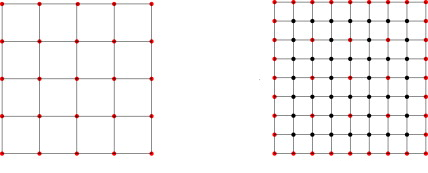
\includegraphics[width=0.6\textwidth]{graphics/fine_grid_vs_coarse_grid.png}
    \caption{An illustrative a coarse and a fine grid}
    \label{fig:coarse_vs_fine_grid}
\end{figure}



\subsubsection*{\textit{Dissertation Structure and Goals}}

Having motivated the investigation of MLMC for SPDEs and illustrating
what this entails, we state the goals of this dissertation.

\begin{itemize}
    \item \textbf{To investigate and quantify the cost reductions achievable with MLMC for 
          parabolic SPDEs.} This will be done by implementing MLMC across 
          several classes of parabolic SPDEs and comparing costs to the baseline method,
          chosen to be the standard Monte Carlo estimator.
    \item \textbf{Investigate different coupling strategies for parabolic SPDEs.}
          This goal is heavily related to the first, as the extent to which coupling 
          is achieved is a determinant in the cost reduction achievable. We will propose
          and investigate several coupling strategies.
    \item \textbf{Assess further performance improvements achievable through high-
          performance implementations}.
          Monte Carlo methods are described as "embarrassingly parallel", lending 
          themselves to implementations on graphics processing units (GPUs). 
          Having assessed the cost reduction of MLMC compared to baseline Monte Carlo 
          methods, we will determine what performance improvements are
          realisable when taking advantage of the highly parallelisable nature of Monte 
          Carlo methods.
\end{itemize}

The structure of this dissertation will be as follows. In the next section we will 
give a theoretical background relevant topics in this dissertation. This will cover 
the main theory of MLMC, a sufficiently relevant overview of SPDEs and a literature
review of the current landscape.

Section SECTION HERE will then present an MLMC implementation for the 
stochastic heat equation. We  validate this implementation through a series of methods, 
varying the quantity of interest being derived, that our MLMC implementation 
converges to this and that its rate of convergence is appropriate. We then 
further validate our MLMC implementation of the Dean-Kawasaki equation, replicating 
the results of the original paper and our implementation.

Section SECTION HERE then presents results for timings. These are 


Section SECTION HERE will present the high performance implementations. 

We finally conclude, outlining further avenues of investigation and telling everyone
great we are.


\section{Prerequisites}

\subsection{Multilevel Monte Carlo}

The MLMC method, introduced by Giles \cite{giles2008multilevel}, is a variance reduction technique
designed to substantially reduce the computational cost of estimating expectations arising from stochastic systems
compared to the standard Monte Carlo method.

Given some quantity $P$, the standard Monte Carlo estimate of $\mathbb{E}\left[P\right]$ 
is given by the average of $N$ independent samples of $P$:

\begin{equation*}
    \mathbb{E}\left[P\right] \approx \frac{1}{N} \sum_{n=1}^{N} P^{(n)} = \hat{P}_{MC}
\end{equation*}

The variance of this estimate is $N^-1 \mathbb{V}\left[P\right]$, therefore the standard error is 
$O(N^{\frac{1}{2}})$ and consequently to achieve an accuracy of $\varepsilon$, $N = O(\varepsilon^{-2})$ samples 
are required.

The treatment above assumes that each Monte Carlo sample $P^{(n)}$ is an exact evaluation of the quantity $P$.
In Practice, however, such evaluations are rarely possible. Typically the quantity of interest $P$ is a functional
of some unknown solution $u(x,t)$ and $u$ is governed by some differential
equation. In this dissertation, this will be 
the case, as $u(x,t)$ will be governed by an SPDE. Since analytic solutions of SPDEs are seldom available, 
numerical methods such as finite-difference or finite-element schemes must be employed. Consequently,
each sample $P_h^{(n)}$ is subject not only to statistical sampling error, but also to a bias or discretisation error
stemming from the finite numerical resolution of the underlying mesh, characterised by a mesh size $h$.
A common measure of the accuracy of Monte Carlo estimates is the Mean  Square Error (MSE). It can be shown that 
the MSE accounts for both the bias in the estimator and its variance. The Root Mean Square Error is also 
commonly employed.


\begin{equation}\label{eq:MSE}
    \text{MSE} \equiv \mathbb{E}\left[(P_h - \mathbb{E}\left[P\right])^2\right] 
    = \underbrace{(\mathbb{E}[P_h] - \mathbb{E}[P])^2}_{\text{Bias}^2}
    \;+\;
    \underbrace{\mathbb{V}[\hat{P}]}_{\text{Variance}}.
\end{equation}

This distinction is fundamental. Simply increasing the number of Monte Carlo samples cannot reduce 
discretisation bias;
only mesh refinement (reducing $h$) can achieve this. Conversely, reducing variance requires larger $N$, 
i.e. more samples. The motivation behind the Multilevel Monte Carlo method is to balance these 
competing requirements efficiently. To achieve this, MLMC leverages a heirarchy of discretisation 
to simultaneously control both bias and variance at significantly reduced computational cost.

MLMC introduces multiple discretisation levels, denotes by mesh sizes $h_\ell = M^{-\ell}h_0$ for 
$\ell = 0, 1, ..., L$ with $M \geq 2$. At each level $\ell$, let $P_\ell$ denote the numerical approximation
of quantity $P$. Then, exploiting the linearity of expectation, one can obtain the following telescoping
sum:

\begin{equation}\label{eq:telescoping_sum}
    \mathbb{E}\left[P_L\right] = \mathbb{E}\left[P_0\right]  + 
    \sum_{\ell = 1}^{L} \mathbb{E}\left[P_\ell - P_{\ell - 1}\right]
\end{equation}

By obtaining a Monte Carlo estimate for each term, equation \eqref{eq:telescoping_sum} brings us to the 
MLMC estimator:

\begin{equation}\label{eq:MLMC_estimator}
    \hat{P}_{MLMC} = \frac{1}{N_0}\sum_{n=1}^{N_0} P_0^{(n)} + 
    \sum_{\ell=1}^{L}\frac{1}{N_{\ell}} \sum_{n=1}^{N_\ell} \left(P_\ell^{(n)} - P_{\ell-1}^{(n)}\right)
\end{equation}

\include{chapter2}
\include{conclusions}

%now enable appendix numbering format and include any appendices
\appendix
\include{appendix1}
\include{appendix2}

%next line adds the Bibliography to the contents page
\addcontentsline{toc}{chapter}{Bibliography}
%uncomment next line to change bibliography name to references
%\renewcommand{\bibname}{References}
\bibliography{refs}        %use a bibtex bibliography file refs.bib
\bibliographystyle{plain}  %use the plain bibliography style

\end{document}
